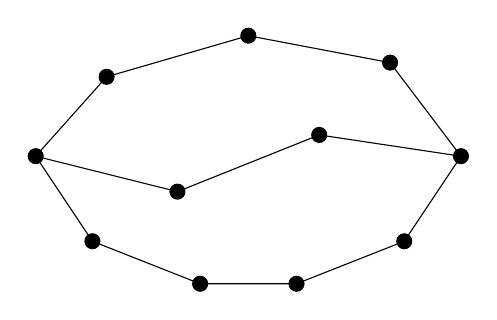
\begin{tikzpicture}[scale=1.8]
\coordinate (a) at (0,0);
\coordinate (b) at (3,0);
\coordinate (c1) at (1,-0.25);
\coordinate (c2) at (2,0.15);
\coordinate (d1) at (2/4,0.56);
\coordinate (d2) at (6/4,0.85);
\coordinate (d3) at (10/4,0.66);
\coordinate (e1) at (2/5,-0.6);
\coordinate (e2) at (5.8/5,-0.9);
\coordinate (e3) at (9.2/5,-0.9);
\coordinate (e4) at (13/5,-0.6);
\draw (a) -- (c1) -- (c2) -- (b);
\draw (a) -- (d1) -- (d2) -- (d3) -- (b);
\draw (a) -- (e1) -- (e2) -- (e3) -- (e4) -- (b);
\foreach \s in {a,b,c1,c2,d1,d2,d3,e1,e2,e3,e4}
{ \draw[fill=black] (\s) circle (1.5pt);};
\end{tikzpicture}